\documentclass[a4paper]{article}
%\documentclass{report} % Can be article, report, book, anything you want!

\usepackage{vub} % this will automatically set to A4 paper. We're not in the US.
% if, for some obscure reason, you need another format, please file an issue (see further).
\usepackage{hyperref}
\usepackage{float}

% The `vub` package has many options.
% Please read the documentation at https://gitlab.com/rubdos/texlive-vub if you want to learn about them.

% Feel free to mix and match with other packages.


\setlength{\parskip}{1em}
\graphicspath{ {./images/} }
\title{Implementing a benchmark in benchkit}
\subtitle{Performance-Analysis-and-Evaluation}
\faculty{Sciences and Bio-Engineering Sciences} % Note: without the word "Faculty"!
\author{Gérard Lichtert\\
        0557513\\
    \href{mailto:gerard.lichtert@vub.be}{gerard.lichtert@vub.be}
}

\begin{document}
\maketitle

\tableofcontents
\newpage
\section{Introduction}
For this assignment I chose to implement the \href{https://github.com/redis/memtier_benchmark}{memcached} benchmark.
memtier\_benchmark is a high-performance traffic generation tool specifically designed to stress-test NoSQL key-value stores like Redis, Valkey, and Memcached.
While many benchmarks focus on how fast a database can write to a disk, memtier
focuses on high-throughput network I/O and concurrency. It simulates thousands
of simultaneous clients to measure how well a database handles a massive volume
of requests and at what point the response time (latency) begins to degrade. It
is used to check if a new release has not decreased in performance.
The source code for the benchmark and campaign can be found at
\textit{benchkit/benches/memcached/benchmark} and
\textit{benchkit/benches/memcached/campaign} respectively.
\section{Parameters}
The passable parameters to the benchmark are:
\begin{itemize}
	\item server\_port: server port
	\item protocol: type of key-value store
	\item authenticate: authentication values
	\item cluster\_mode: run client in cluster mode
	\item requests: amount of requests or all keys
	\item nb\_clients: Amount of clients per thread
	\item nb\_threads: Amount of threads
	\item run\_count: Amount of runs (unsupported for collection)
	\item test\_time: Limit run by test\_time
	\item pipeline: Number of concurrent pipelined requests
	\item ratio: Ratio of Sets:Gets
	\item key\_pattern: Key pattern for the command
	\item data\_size: Object size in bytes
	\item key\_minimum: Key ID minimum value
	\item key\_maximum: Key ID maximum value
\end{itemize}
Whilst these are not all the possible parameters that can be passed to
\textit{memtier\_benchmark}, these are the most interesting.
I varied my threads from 1 to 12, applied a gaussian distribution to the
key\_pattern and repeated the campaign 30 times (not to be confused with
run\_count)
\section{Captured results}
\label{sec:captured results}
The benchmark not only captures the operations per second, hits per second, misses per second, but
also Average latency, p50 latency, p99 latency, p99.99 latency and KB per
second. It records these for the sets, gets, waits and the total.
\section{Campaign}
The implemented campaign measures the values stated in
\ref{sec:captured results} as well as the amount of instructions, cache misses
and cycles per run. I used a \textit{PerfStatWrapper} and I chose it to try to
see if there was a corrolation between cache misses and amount of threads used,
as well as to see what the IPC is.
\begin{figure}[H]
	\centering
	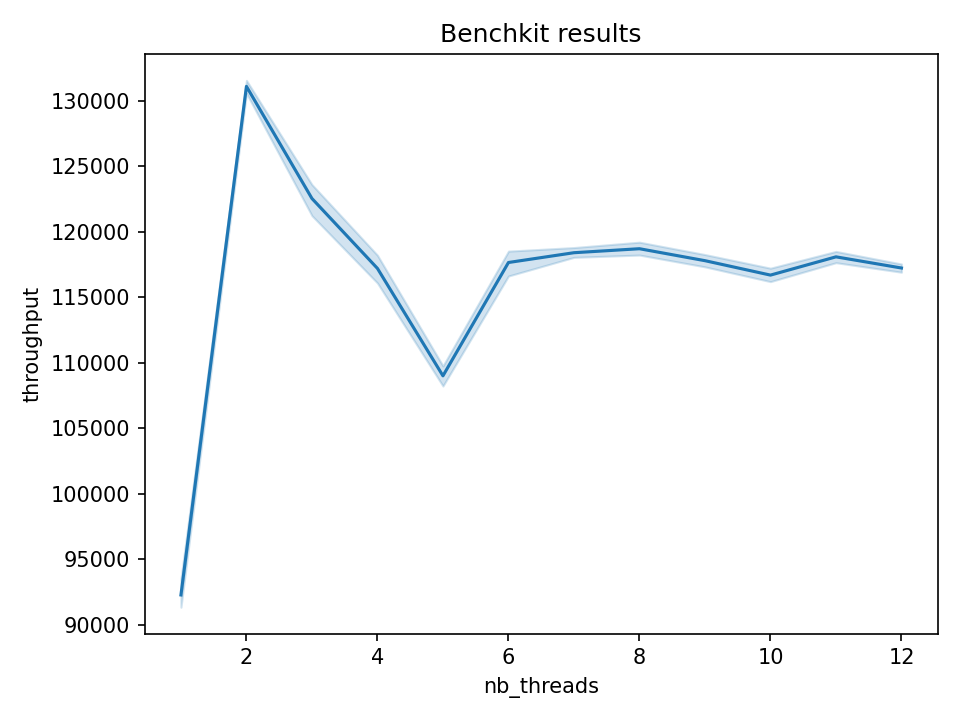
\includegraphics[width=0.7\textwidth]{benchkit-20260510-181942-01.png}
	\caption{throughput given N threads}
	\label{fig:throughput given n threads}
\end{figure}
In \ref{fig:throughput given n threads} we can see that the throughput rises at
first but then drops before stabilizing. Whilst there is an optimization to be
made by using more than one thread, it seems that there is a limit in how much
performance can be gained by adding threads, as per Amdahls law. Notably
however, the speedup is quite poor starting from a low amount of threads, likely
indicating that it's very tough to parallelize or that the majority is
sequential.
\begin{figure}[H]
	\centering
	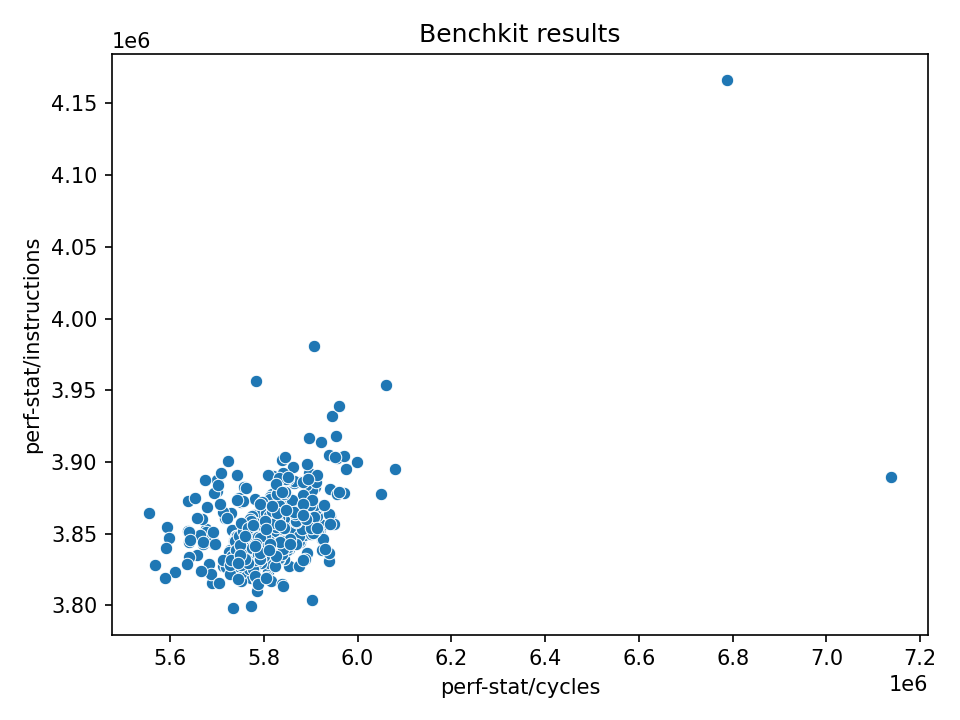
\includegraphics[width=0.7\textwidth]{benchkit-20260510-201800-01.png}
	\caption{Instructions given n cycles}
	\label{fig:instruction given n cycles}
\end{figure}
in \ref{fig:instruction given n cycles} we can see that about 3.85 million
instructions are executed during roughly 5.8 million cycles. This is roughly an
0.66 IPC which is relatively low. This could indicate that the CPU spends a
significant amount of time doing nothing. Likely due to it having to wait for
data from memory due to cache misses. This is not unusual for database related
workloads (such as the key value store this benchmark operates on)
\begin{figure}[H]
	\centering
	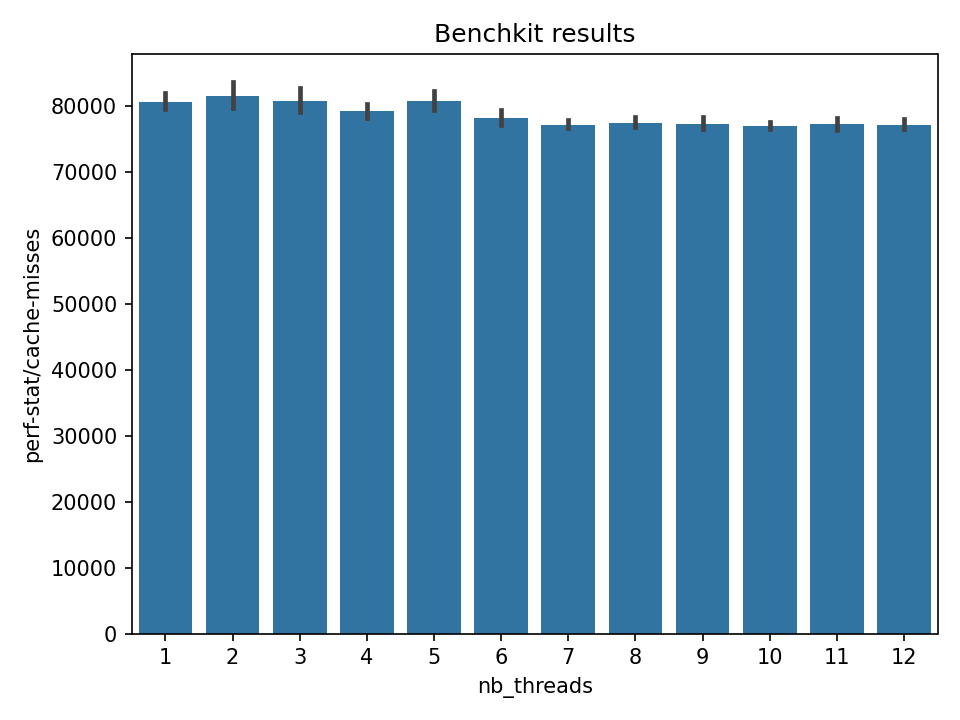
\includegraphics[width=0.7\textwidth]{benchkit-20260510-203049-01.png}
	\caption{cache misses given n threads}
	\label{fig:cache misses given n threads}
\end{figure}
using both \ref{fig:throughput given n threads} and \ref{fig:cache misses given n threads}
we can actually see that of the $\approx$ 115K operations per second (if we
assume a time elapsed of around 10 seconds), there aren't many cache misses.
However, it would perhaps be more interesting to verify which cache is being
missed, as missing in a lower level cache is more expensive than in a higher
one. Regardless, it's not surprising that the IPC is so low, since it is mainly
working with DRAM, which is orders of magnitudes slower than memory in the
caches.
\end{document}
